In this chapter, the details of implementation are discussed. It starts with the introduction of the overview and the architecture of the visualization application, and is followed by describing three important component in the application: the simulator, the watchdog, and the visualizer. In the next section, we provide an UML class diagram and several tables to describe the functionalities of the classes. Finally, the important algorithm about the mining processes is proposed to clearify the operation of mining activities.

\section{Architecture}

\begin{figure}[htb]
    \centering
    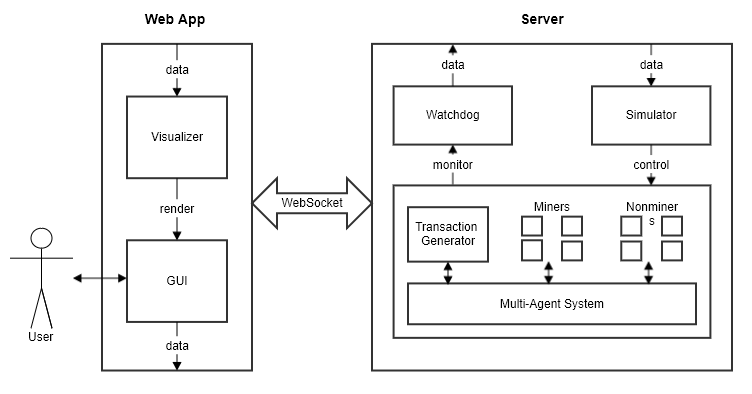
\includegraphics[width=\textwidth]{impl_architecture}
    \caption{Architecture.}
    \label{fig:architecture}
\end{figure}

Figure \ref{fig:architecture} shows the whole architecture of the visualization application. The architecture contains a web app and a server, which are connected with WebSocket. WebSocket technology makes the real-time communications between the web app and the server possible, as the visualization of the real-time mining processes is necessary. The user can interact with the web application through the graphical user interface.

The server maintains the blockchain system. It is composed of three components.

\begin{itemize}
    \item \textbf{Blockchain System} \\
        The blockchain system is based on a multi-agent system. It cointains a transaction generator, multiple miners, and multiple nonminers. The multi-agent system provides communications for these nodes.
    \item \textbf{Simulator} \\
        The simulator is responsible for receiving data from the client side and controlling the blockchain system.
    \item \textbf{Watchdog} \\
        When the blockchain data structures change in the blockchain system, the watchdog will catch these changes, and send them to the web app. 
\end{itemize}

Since the nodes on the blockchain network can be regarded as agents on a multi-agent system, we decided to contruct the blockchain system with a multi-agent system framework. Here, We choose a web-based multi-agent system framework called Eve \cite{eve}. The main features of Eve are stated below.

\begin{itemize}
    \item \textbf{Robustness} \\
        The agents are decoupled and can be maintained independently. Thus, the whole system is still active even an agent fails.
    \item \textbf{Flexibility} \\
        It is flexible to add or remove agents.
    \item \textbf{Reduced complexity} \\
        The complexity of the distributed software design is lower.
    \item \textbf{Scalability} \\
        The limitation of the number of agents does not exist, so the scalability can grow rapidly.
\end{itemize}

In addtion, Eve provides reliable communications with JSON-RPC protocols \cite{jsonrpc}. Therefore, agents can send and understand the JSON format data between each other, and they can be maintained independently in anywhere, e.g., on the cloud or desktops. Eve is an open source project which is implemented in JavaScript, and it is easy to learn. As a result, Eve allows us to construct a distributed blockchain system without worrying about the technical problems such as asynchronous and locking problems.

The server is built in Node.js with Express framework because of it is based on the same programming language of Eve. During the runtime, a transaction generator, miners, and nonminers can be instantiated and destroyed at any time thanks to the flexibility of Eve.

The web application is responsible for the visualization and the interactions with users. There are two components in the web application.

\begin{itemize}
    \item \textbf{Visualizer} \\
        The visualizer is responsible for rendering the visualization of blockchains when it is notified by the watchdog. It receives the data of transactions and blocks from the server and renders them appropriately on the HTML documents.
    \item \textbf{Graphical User Interface} \\
        The GUI provides an index page and a settings page. The index page is for the visualization part, and the settings page displays all the defined parameters in the blockchain system. More details can be refered to Section \ref{sec:flow}.
\end{itemize}

The visualization is based on Three.js, a JavaScript framework for rendering 2D and 3D graphics. Three.js uses WebGL as the renderer, and the updating performance is 60 frame per second. The reason to choose Three.js as the visualization framework is that it is an famous open source project, and the community is active. Moreover, Three.js provides basic shapes, e.g., squares and lines, and handles the updating of frames. Therefore, we can focus on optimize the user experience of the visualization without considering the implementation of WebGL.

\section{Simulator}

The simulator is responsible for controlling the blockchain system and handling all the requests from the client. It is unique in the whole system, so it observes to the singleton pattern. The role of the simulator is like a "door" as it is the only gate to communicate with the blockchain system.

After the blockchain system starts, the simulator initializes the status of the blockchain system, i.e., it instantiates necessary nodes according to the configuration. The waiting list of transactions in the transaction generator and the blockchain data structures of miners and nonminers are initialized by the simulator. 

When the user wants to change the parameters, i.e., the mining strategy and delays of networks, or the visualizer needs the information of transaction pools and blockchains, the simulator will interact with the blockchain system by setting the parameters or retrieving the required data. The data are sent through WebSocket in real-time.

The simulator is an important component because it hides the details of the implementation of the blockchain system and provides a unique and robust interface for the requests from the client. As a result, it decouples the relationship between the web application and the blockchain system. The detail of the simulator can be refered to \ref{sec:uml diagram}.

\section{Watchdog}

The watchdog is responsible for monitoring the behaviors of nodes and notifying the visualizer when the data should be updated. It is unique in the whole system, so it also observes to the singleton pattern.

The watchdog watches three kinds of data in the blockchain system.

\begin{itemize}
    \item blockchain data structures
    \item status of transaction pools
    \item status of mining
\end{itemize}

While a miner receives a transaction or a block, a nonminer receives a block, or a miner is solving the puzzle, the watchdog will notify the visualizer in real-time through WebSocket. Therefore, it is guaranteed that the visualization of the data is synchronized with the blockchain system all the time.

With the help of the watchdog, the activities that happened in the blockchain system is recorded completely. Hence, it ensures the correctness of the visualization application. The detail of the watchdog can be refered to \ref{sec:uml diagram}.

\section{Visualizer}

The visualizer is responsible for rendering the data that are sent from the watchdog. It is the main part of the visualization application because it shows the elegance of visualization. 

Three items are updated by the visualizer continuously.

\begin{itemize}
    \item status bars for transaction pools
    \item status bars for mining
    \item blockchain data structures
\end{itemize}

The status bars for transaction pools and the status bars for mining are auxiliary tools to help the user understand the events that are acctually happening in mining activities. The status bar for transaction pools becomes longer if the pending transactions are growing and vice versa. The status barsfor mining is usually empty, except that the miner is solving the puzzle. It increases each second when the mining activity continuouses. Unlike the real blockchain networks, the time of solving the puzzles is predictable in our visualization application, and it is defined in the parameter of the mining strategy. The main area of the visualization is reserved for the blockchain data structures. Squares represent blocks, and they are chained by lines. Different colors of the squares represent the different sources of the blocks. The growth of the blockchain data structures is dynamic and real-time as the mining activities are in progress.

The visualizer expresses fantastic blockchain visualization that is able to attract the user. In addition, it explains the steps of mining processes understandably, even for the viewers who are new to blockchain technology. The detail of the visualizer can be refered to \ref{sec:uml diagram}.

\section{UML Diagram}
\label{sec:uml diagram}

In Figure \ref{fig:class diagram}, it demonstrates the class diagram of the visualization application. The blockchain system is based on the multi-agent system framework Eve. Abstract class \texttt{AbstractNode} inherits from \texttt{Agent} in Eve, and class \texttt{TransactionGenerator}, class \texttt{Miner}, and class \texttt{Nonminer} inherit from it. The blockchain system is controlled by class \texttt{Simulator}, and class \texttt{Watchdog} monitors it and notify class \texttt{Visualizer} when it is necessary to update. Class \texttt{GUI} provides the user interface and is able to interact with \texttt{Simulator}. Finally, a helper class \texttt{Hash} provides simulation functionalities of the hash computation. The following contains all the classes that compose the visualization application.

\begin{itemize}
    \item \textbf{Agent} (Table \ref{tab:class agent}) \\
        \texttt{Agent} is from the multi-agent system framework, Eve. It establishes the communication channel for the agents. In the implementation, the channel is opened with HTTP protocols. It makes sending and receiving transactions and blocks very simple. 
    \item \textbf{AbstractNode} (Table \ref{tab:class abstractNode}) \\
        It defines the common properties and methods of its children. \texttt{AbstractNode} is an abstract class, so it is not allowed to instantiate instances from it. In contrast, we can create nodes from the children of \texttt{AbstractNode}, i.e., \texttt{TransactionGenerator}, \texttt{Miner}, and \texttt{Nonminer}
    \item \textbf{TransactionGenerator} (Table \ref{tab:class transactiongenerator}) \\
        It is responsible for generating and publishing transactions. There should be only one transaction generator in the blockchain system. Furthermore, the neighbors of the transaction generator only contain the miners.
    \item \textbf{Miner} (Table \ref{tab:class miner}) \\
        \texttt{Miner} is the main role in the blockchain system. It generates and publishes blocks through the blockchain network. Therefore, it controls all the mining processes in the blockchain system.
    \item \textbf{Nonminer} (Table \ref{tab:class nonminer}) \\
        \texttt{Nonminer} represents common users who do not solve complex mathematical puzzles in the blockchain system. The only behavior of nonminers is to receive and publish blocks. Consequently, the miners and the nonminers connect with each other. 
    \item \textbf{Simulator} (Table \ref{tab:class simulator}) \\
        \texttt{Simulator} is the only master of the blockchain system. It is able to add and update nodes, and retrieve information from the blockchain system.
    \item \textbf{Watchdog} (Table \ref{tab:class watchdog}) \\
        \texttt{Watchdog} monitors the blockchain system. When a mining activity starts, it keeps notifying the visualizer until the end.
    \item \textbf{Visualizer} (Table \ref{tab:class visualizer}) \\
        \texttt{Visualizer} uses 3D graphical library to render the blockchain visualization. It maintains all miners' and nonminers' canvases and the mouse events which enable users to drag, zoom in, and zoom out the canvases.
    \item \textbf{GUI} (Table \ref{tab:class gui}) \\
        The graphical user interface is responsible for the interactions with users, including uploading files, updating the blockchain sytem, publishing transactions, and resetting the blockchain system.
    \item \textbf{Hash} (Table \ref{tab:class hash}) \\
        This class generates a sequence of random numbers to simulate the hash functions. It avoids to put lots of computing resources to calculate hash values.
\end{itemize}

\section{Algorithms}
\label{sec:algorithms}

The visualization focuses on the mining processes, i.e., generating and publishing blocks. Hence, the algorithm about mining processes is the key parts of the entire system. The algorithm can be divided into three parts.

\begin{itemize}
    \item Select Candidate Transactions
    \item Mining
    \item Add Block to Blockchain
\end{itemize}

Before a miner starts to mine a block, he/she needs to select a set of candidate transactions for the transaction pool. Thus, these candidate transactions serve as the content of the mined block. After receiving a block, the node will check the layer of the new block, and switch to the new block if the blockchain becomes the longest.

In Algorithm \ref{alg:select candidate transactions}, it states the procedure of selecting a set of candidate transactions. Assume the pending transactions in the transaction pool are sorted according to their values. There are two cases at the beginning of the algorithm. ``Maximum number of pending transactions'' is defined in the parameters of the mining strategy.

\begin{enumerate}
    \item \textbf{the number of pending transactions in the transaction pool $\geq$ maximum number of pending transactions} \\
        Because the mining strategy does not allow appending more pending transactions into the transaction pool, the miner must select a set of pending transactions. The minimum value of transactions, a parameter of mining strategy, is ignored here. Consequently, the miner will select from the transaction with the highest value, until the number of candidate transactions is enough for mining a block.
    \item \textbf{the number of pending transactions in the transaction pool < maximum number of pending transactions} \\
        In this case, the miner selects transactions which values are higher than the minimum value of transactions.
\end{enumerate}

In both cases, if a transaction is not selected as a candidate transaction, then the privilege of the transaction will increase. Finally, if the number of selected candidate transactions is larger than the number of transactions to be mined, then the miner will start to mine a block. Otherwise, the miner will put the candidate transactions back into the transaction pool and give up to mine a block.

Regarding the mining algorithm (Algorithm \ref{alg:mining}), it simulates the process of solving a puzzle in the proof-of-work base blockchain system. After determining the candidate transactions, the miner starts a timer until it meets the duration of time that should be spent on mining. That is, it means that the miner solves the puzzle successfully. Thus, the miner is ready for generating and publishing the block.

Receiving a new block triggers the consensus protocol to resolve the longest blockchain (Algorithm \ref{alg:add block to blockchain}). There are two cases that will happen when receiving a new block.

\begin{enumerate}
    \item \textbf{the id of the previous block of the new block is empty} \\
        It happens because the new block was mined by the miner himself/herself. Therefore, the miner puts the new block on the top of the current blockchain, i.e., the miner adds the new block after the current block.
    \item \textbf{the id of the previous block of the new block is not empty} \\
        The consensus protocol is very simple because we do not consider malicious nodes in the blockchain system currently. If the received block is at a higher layer, i.e., the blockchain becomes longer, then the node will switch the current block to the received block to ensures that it is working on the correct blockchain. Moreover, the transactions of the received block are deleted from the transaction pools because these transactions are not pending anymore.
\end{enumerate}

Last, the node publishes the received block through the blockchain network to make sure that every neighbor has the same blockchain data structure. In addition, the miner calculates and updates his/her total rewards if the blockchain becomes longer.

\clearpage

\begin{figure}[!ht]
    \centering
    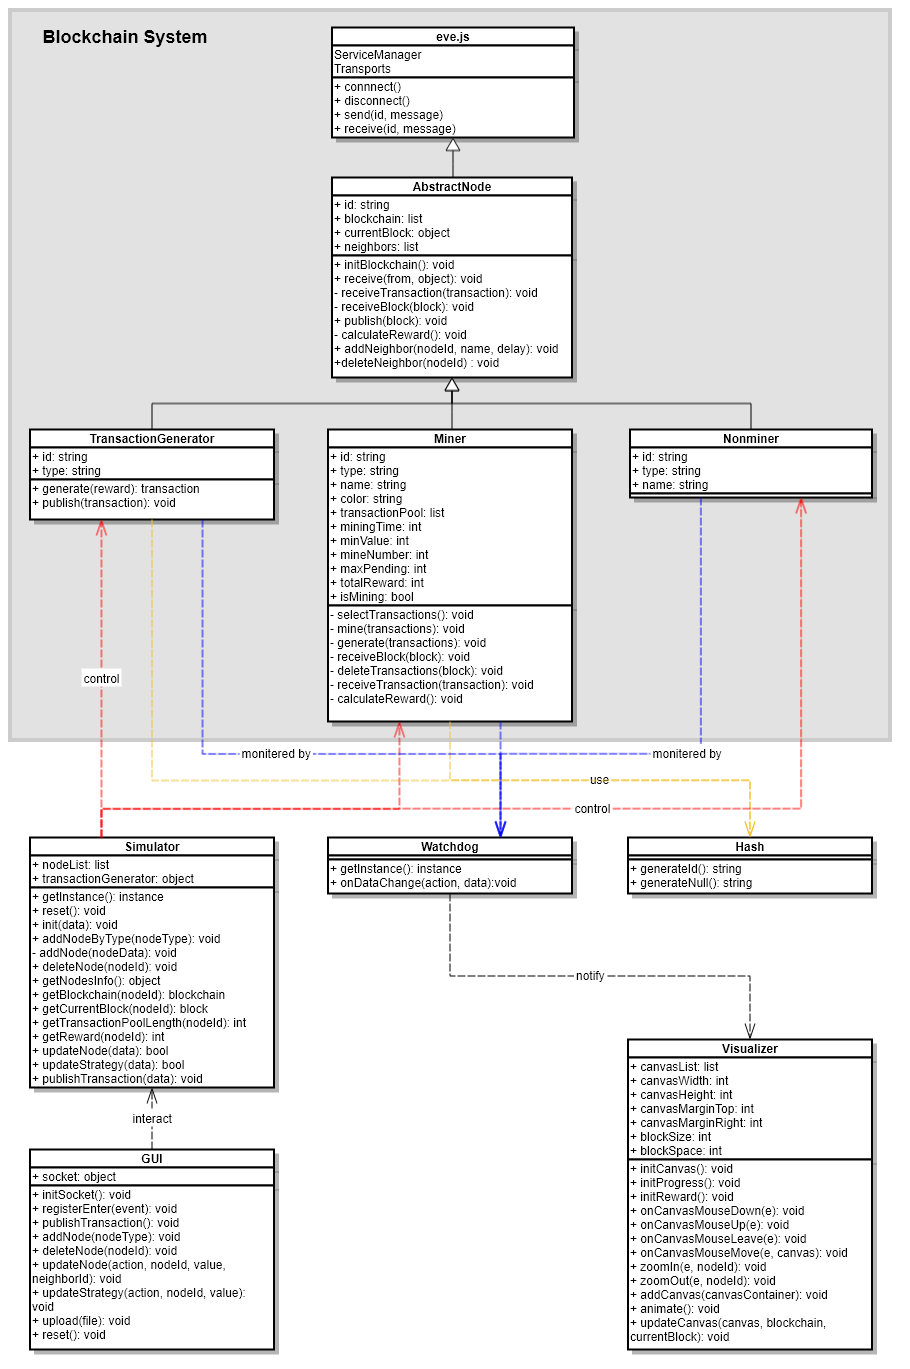
\includegraphics[width=\textwidth]{impl_uml}
    \caption{Class Diagram.}
    \label{fig:class diagram}
\end{figure}

\begin{table}[!ht]
    \centering
    \begin{tabular}{ M{3.5cm}|m{8cm} } 
        \hline
        \multicolumn{2}{c}{\textbf{Agent (eve.js)}} \\
        \hline
        \textit{Properties} & \multicolumn{1}{c}{\textit{Description}} \\
        \hline
        transport & communication channels. \\ 
        \hline
        \textit{Methods} & \multicolumn{1}{c}{\textit{Description}} \\
        \hline
        connect & connect with a transport. \\ 
        disconnect & disconnect from a transport. \\ 
        send & send messages to a transport. \\ 
        receive & receive messages from a transport. \\ 
        \hline
    \end{tabular}
    \caption{Class \texttt{Agent}}
    \label{tab:class agent}
\end{table}

\begin{table}[!ht]
    \centering
    \begin{tabular}{ M{3.5cm}|m{8cm} } 
        \hline
        \multicolumn{2}{c}{\textbf{AbstractNode}} \\
        \hline
        \textit{Properties} & \multicolumn{1}{c}{\textit{Description}} \\
        \hline
        id & unique in the multi-agent system. \\ 
        blockchain & blockchain data structures. \\ 
        currentBlock & the id of the block which is on the top of the longest blockchain. \\ 
        neighbors & reachable nodes. \\ 
        \hline
        \textit{Methods} & \multicolumn{1}{c}{\textit{Description}} \\
        \hline
        initBlockchain & initialize blockchain data structures. \\ 
        receive & inherit from \texttt{eve.js}. \\ 
        receiveTransaction & define actions of receiving transactions. \\ 
        receiveBlock & define actions of receiving blocks. \\ 
        publish & publish transactions or blocks. \\ 
        calculateReward & calculate the total mining rewards. \\ 
        addNeighbor & add a new node as a neighbor. \\ 
        deleteNeighbor & delete a node from neighbors. \\ 
        \hline
    \end{tabular}
    \caption{Class \texttt{AbstractNode}}
    \label{tab:class abstractNode}
\end{table}

\begin{table}[!ht]
    \centering
    \begin{tabular}{ M{3.5cm}|m{8cm} } 
        \hline
        \multicolumn{2}{c}{\textbf{TransactionGenerator}} \\
        \hline
        \textit{Properties} & \multicolumn{1}{c}{\textit{Description}} \\
        \hline
        id & unique in the multi-agent system. \\ 
        type & is always ``generator''. \\ 
        \hline
        \textit{Methods} & \multicolumn{1}{c}{\textit{Description}} \\
        \hline
        generate & generate a transaction. \\ 
        publish & publish a transaction. \\ 
        \hline
    \end{tabular}
    \caption{Class \texttt{TransactionGenerator}}
    \label{tab:class transactiongenerator}
\end{table}

\begin{table}[!ht]
    \centering
    \begin{tabular}{ M{3.5cm}|m{8cm} } 
        \hline
        \multicolumn{2}{c}{\textbf{Miner}} \\
        \hline
        \textit{Properties} & \multicolumn{1}{c}{\textit{Description}} \\
        \hline
        id & unique in the multi-agent system. \\ 
        type & is always ``miner''. \\ 
        name & a simple nickname. \\ 
        color & the color of the generated blocks. \\ 
        transactionPool & contain pending transactions. \\ 
        miningTime & computing power. \\ 
        minValue & minimum value of transactions. \\ 
        mineNumber & size of blocks. \\ 
        maxPending & maximum pending transactions. \\ 
        totalReward & total number of rewards. \\ 
        isMining & whether the miner is mining. \\ 
        \hline
        \textit{Methods} & \multicolumn{1}{c}{\textit{Description}} \\
        \hline
        selectTransactions & select pending transactions as candidates. \\ 
        mine & solve the puzzles. \\ 
        generate & generate a block instance. \\ 
        receiveBlock & inherit from \texttt{AbstractNode}. \\ 
        deleteTransactions & delete mined transactions from the transaction pool. \\ 
        receiveTransaction & inherit from \texttt{AbstractNode}. \\ 
        calculateReward & inherit from \texttt{AbstractNode}. \\ 
        \hline
    \end{tabular}
    \caption{Class \texttt{Miner}}
    \label{tab:class miner}
\end{table}

\begin{table}[!ht]
    \centering
    \begin{tabular}{ M{3.5cm}|m{8cm} } 
        \hline
        \multicolumn{2}{c}{\textbf{Nonminer}} \\
        \hline
        \textit{Properties} & \multicolumn{1}{c}{\textit{Description}} \\
        \hline
        id & unique in the multi-agent system. \\ 
        type & is always ``nonminer''. \\ 
        name & a simple nickname. \\ 
        \hline
    \end{tabular}
    \caption{Class \texttt{Nonminer}}
    \label{tab:class nonminer}
\end{table}

\begin{table}[!ht]
    \centering
    \begin{tabular}{ M{3.5cm}|m{8cm} } 
        \hline
        \multicolumn{2}{c}{\textbf{Simulator}} \\
        \hline
        \textit{Properties} & \multicolumn{1}{c}{\textit{Description}} \\
        \hline
        nodeList & a list of all nodes. \\ 
        transactionGenerator & reference to the transaction generator. \\ 
        \hline
        \textit{Methods} & \multicolumn{1}{c}{\textit{Description}} \\
        \hline
        getInstance & get the instance of the simulator. \\ 
        reset & reset the blockchain system. \\ 
        init & initialize the blockchain system. \\ 
        addNodeByType & add a new node with defined type. \\ 
        addNode & add a new node. \\ 
        deleteNode & delete a node. \\ 
        getNodesInfo & get the information of a node. \\ 
        getBlockchain & get the blockchain data structure of a node. \\ 
        getCurrentBlock & get the information of the current block of a node. \\ 
        \begin{tabular}[c]{@{}c@{}}getTransactionPool- \\ Length\end{tabular} & get the level of capacity of the transaction pool of a node. \\ 
        getReward & get the number of rewards of a node. \\ 
        updateNode & update the information of a node. \\ 
        updateStrategy & update the parameters of the mining strategy of a node. \\ 
        publishTransaction & publish a transaction through the transaction generator. \\ 
        \hline
    \end{tabular}
    \caption{Class \texttt{Simulator}}
    \label{tab:class simulator}
\end{table}

\begin{table}[!ht]
    \centering
    \begin{tabular}{ M{3.5cm}|m{8cm} } 
        \hline
        \multicolumn{2}{c}{\textbf{Watchdog}} \\
        \hline
        \textit{Methods} & \multicolumn{1}{c}{\textit{Description}} \\
        \hline
        getInstance & get the instance of the watchdog. \\ 
        onDataChange & monitoring the data. \\ 
        \hline
    \end{tabular}
    \caption{Class \texttt{Watchdog}}
    \label{tab:class watchdog}
\end{table}

\begin{table}[!ht]
    \centering
    \begin{tabular}{ M{3.5cm}|m{8cm} } 
        \hline
        \multicolumn{2}{c}{\textbf{Visualizer}} \\
        \hline
        \textit{Properties} & \multicolumn{1}{c}{\textit{Description}} \\
        \hline
        canvasList & a list of all canvases. \\ 
        canvasWidth & the width of each canvas. \\ 
        canvasHeight & the height of each canvas. \\ 
        canvasMarginTop & the top margin of each canvas. \\ 
        canvasMarginRight & the right margin of each canvas. \\ 
        blockSize & the size of blocks. \\ 
        blockSpace & the spaces between blocks. \\ 
        \hline
        \textit{Methods} & \multicolumn{1}{c}{\textit{Description}} \\
        \hline
        initCanvas & initialize all canvases. \\ 
        initProgress & initialize progress bars. \\ 
        initReward & initialize the numbers of rewards. \\ 
        onCanvasMouseDown & mouse event. \\ 
        onCanvasMouseUp & mouse event. \\ 
        onCanvasMouseLeave & mouse event. \\ 
        onCanvasMouseMove & mouse event. \\ 
        zoomIn & zoom in with mouse. \\ 
        zoomOut & zoom out with mouse. \\ 
        addCanvas & add a new canvas. \\ 
        animate & update by each frame. \\ 
        updateCanvas & update a canvas. \\ 
        \hline
    \end{tabular}
    \caption{Class \texttt{Visualizer}}
    \label{tab:class visualizer}
\end{table}

\begin{table}[!ht]
    \centering
    \begin{tabular}{ M{3.5cm}|m{8cm} } 
        \hline
        \multicolumn{2}{c}{\textbf{GUI}} \\
        \hline
        \textit{Properties} & \multicolumn{1}{c}{\textit{Description}} \\
        \hline
        socket & the instance of WebSocket. \\ 
        \hline
        \textit{Methods} & \multicolumn{1}{c}{\textit{Description}} \\
        \hline
        initSocket & initialize WebSocket. \\ 
        registerEnter & register enter keyboard. \\ 
        publishTransaction & publish a transaction. \\ 
        addNode & add a new node. \\ 
        deleteNode & delete a node. \\ 
        updateNode & update a node. \\ 
        updateStrategy & update the parameters of the mining strategy of a node. \\ 
        upload & upload a configuration file. \\ 
        reset & reset the blockchain system. \\ 
        \hline
    \end{tabular}
    \caption{Class \texttt{GUI}}
    \label{tab:class gui}
\end{table}

\begin{table}[!ht]
    \centering
    \begin{tabular}{ M{3.5cm}|m{8cm} } 
        \hline
        \multicolumn{2}{c}{\textbf{Hash}} \\
        \hline
        \textit{Methods} & \multicolumn{1}{c}{\textit{Description}} \\
        \hline
        generateId & generate a hash value for id. \\ 
        generateNull & generate a hash value only with zeros. \\ 
        \hline
    \end{tabular}
    \caption{Class \texttt{Hash}}
    \label{tab:class hash}
\end{table}

\begin{algorithm}[!ht]
    \caption{Select Candidate Transactions}
    \label{alg:select candidate transactions}
\begin{algorithmic}[1]
    \Procedure{Select Transactions}{}
    \State candidateTransactions $\gets$ empty
    \State
    \If{transactionPool.length $\geq$ maximum number of pending transactions}
        \ForAll{pending transaction}
            \If{candidateTransactions.length $<$ \\ 
                \hspace{\algorithmicindent}\hspace{\algorithmicindent}\hspace{\algorithmicindent}number of transactions to be mined}
                \State add this transaction to candidateTransactions
                \State remove this transaction from transaction pool
            \Else
                \State add the privilege of this transaction by 1
            \EndIf
        \EndFor
    \ElsIf{transactionPool.length $\geq$ number of transactions to be mined}
        \ForAll{pending transaction}
            \State value $\gets$ reward $+$ privilege
            \If{value $>$ minimum value of transactions \textit{AND} \\ 
            \hspace{\algorithmicindent}\hspace{\algorithmicindent}\hspace{\algorithmicindent} candidateTransactions.length $<$ number of transactions to be mined}
                \State add this transaction to candidateTransactions
                \State remove this transaction from transaction pool
            \Else
                \State add the privilege of this transaction
            \EndIf
        \EndFor
    \EndIf
    \State
    \If{candidateTransactions.length $=$ number of transactions to be mined}
        \State \Call{Mine}{candidateTransactions}
    \Else
        \State add candidateTransactions to pending transactions
    \EndIf
    \State
    \State notify watchdog
    \EndProcedure
\end{algorithmic}
\end{algorithm}

\begin{algorithm}[!ht]
    \caption{Mining}
    \label{alg:mining}
\begin{algorithmic}[1]
    \Procedure{Mine}{candidateTransactions}
    \State count $\gets$ 0
    \State isMining $\gets$ true
    \State
    \Repeat 
    \State count += 1
    \State notify watchdog
    \Until{count $\geq$ mining time}
    \State
    \State isMining $\gets$ false
    \State block $\gets$ \Call{generate}{candidateTransactions}
    \State \Call{receiveBlock}{block}
    \State notify watchdog
    \EndProcedure
\end{algorithmic}
\end{algorithm}

\begin{algorithm}[!ht]
    \caption{Add Block to Blockchain}
    \label{alg:add block to blockchain}
\begin{algorithmic}[1]
    \Procedure{Receive Blocks}{block}
    \If{block.previous $=$ none}
        \State block.previous $\gets$ currentBlock.id
        \State block.layer $\gets$ currentBlock.layer + 1
        \State currentBlock $\gets$ block
        \State delete the mined transactions from transaction pool
    \ElsIf{currentBlock.layer $<$ block.layer}
        \State currentBlock $\gets$ block
        \State delete the mined transactions from transaction pool
    \EndIf
    \State
    \State add block to blockchain
    \State publish block to neighbors
    \State calculate the total rewards
    \State notify watchdog
    \EndProcedure
\end{algorithmic}
\end{algorithm}
